\documentclass{article}
\usepackage{amsmath,amssymb}
\usepackage{tikz}
\usetikzlibrary{shapes.geometric,arrows.meta,positioning,calc,fit,backgrounds}
\usepackage[paperwidth=18cm,paperheight=8.6cm,margin=0.2cm]{geometry}
\pagestyle{empty}

\begin{document}
\noindent
\centering
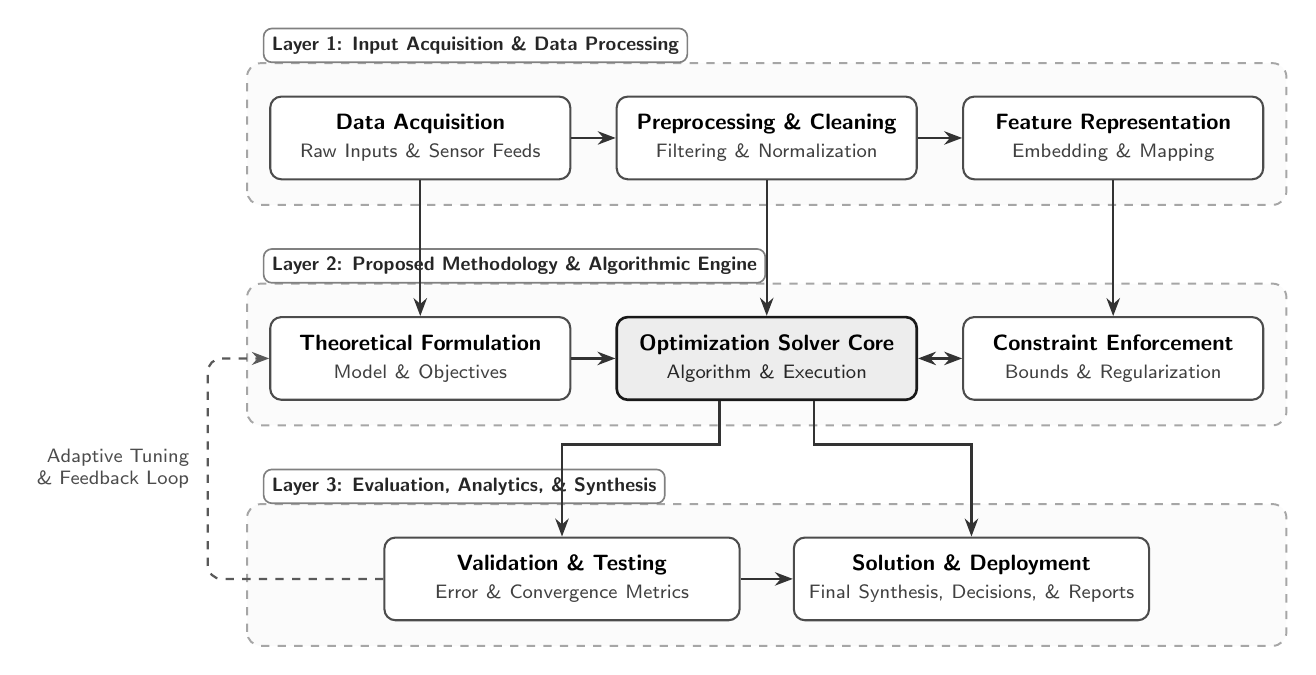
\begin{tikzpicture}[
    auto,
    >=Stealth,
    font=\sffamily,
    % Layer Box Style
    layerbox/.style={
        draw=black!35,
        fill=black!1.5,
        dashed,
        rounded corners=5pt,
        line width=0.7pt
    },
    layertitle/.style={
        fill=white,
        draw=black!50,
        rounded corners=3pt,
        line width=0.6pt,
        font=\fontsize{7.5pt}{8.5pt}\selectfont\bfseries\sffamily,
        text=black!85,
        inner sep=3pt
    },
    % Component Card Styles with tight, proportional linespacing
    card/.style={
        rectangle,
        draw=black!70,
        fill=white,
        rounded corners=4pt,
        line width=0.75pt,
        minimum width=3.8cm,
        minimum height=1.05cm,
        text width=3.6cm,
        align=center,
        inner sep=3pt,
        font=\fontsize{8.5pt}{9.5pt}\selectfont\sffamily
    },
    corecard/.style={
        rectangle,
        draw=black!90,
        fill=black!7,
        rounded corners=4pt,
        line width=0.95pt,
        minimum width=3.8cm,
        minimum height=1.05cm,
        text width=3.6cm,
        align=center,
        inner sep=3pt,
        font=\fontsize{8.5pt}{9.5pt}\selectfont\sffamily
    },
    widecard/.style={
        rectangle,
        draw=black!70,
        fill=white,
        rounded corners=4pt,
        line width=0.75pt,
        minimum width=4.5cm,
        minimum height=1.05cm,
        text width=4.3cm,
        align=center,
        inner sep=3pt,
        font=\fontsize{8.5pt}{9.5pt}\selectfont\sffamily
    },
    % Arrow Styles
    arrow/.style={
        ->,
        >={Stealth[scale=0.95]},
        line width=0.85pt,
        draw=black!80
    },
    biarrow/.style={
        <->,
        >={Stealth[scale=0.95]},
        line width=0.85pt,
        draw=black!80
    },
    feedback/.style={
        ->,
        >={Stealth[scale=0.95]},
        line width=0.8pt,
        draw=black!65,
        dashed,
        rounded corners=5pt
    }
]

    % =========================================================================
    % LAYER 1: DATA INGESTION & PREPARATION (y = 5.5)
    % =========================================================================
    \node[card] (data_raw) at (-4.4, 5.5) {%
        \textbf{Data Acquisition}\\[0.5pt]%
        {\fontsize{7.2pt}{8.2pt}\selectfont\color{black!75}Raw Inputs \& Sensor Feeds}%
    };

    \node[card] (data_prep) at (0, 5.5) {%
        \textbf{Preprocessing \& Cleaning}\\[0.5pt]%
        {\fontsize{7.2pt}{8.2pt}\selectfont\color{black!75}Filtering \& Normalization}%
    };

    \node[card] (data_feat) at (4.4, 5.5) {%
        \textbf{Feature Representation}\\[0.5pt]%
        {\fontsize{7.2pt}{8.2pt}\selectfont\color{black!75}Embedding \& Mapping}%
    };

    \draw[arrow] (data_raw) -- (data_prep);
    \draw[arrow] (data_prep) -- (data_feat);

    % =========================================================================
    % LAYER 2: COMPUTATIONAL CORE & METHODOLOGY (y = 2.7)
    % =========================================================================
    \node[card] (core_form) at (-4.4, 2.7) {%
        \textbf{Theoretical Formulation}\\[0.5pt]%
        {\fontsize{7.2pt}{8.2pt}\selectfont\color{black!75}Model \& Objectives}%
    };

    \node[corecard] (core_solver) at (0, 2.7) {%
        \textbf{Optimization Solver Core}\\[0.5pt]%
        {\fontsize{7.2pt}{8.2pt}\selectfont\color{black!85}Algorithm \& Execution}%
    };

    \node[card] (core_const) at (4.4, 2.7) {%
        \textbf{Constraint Enforcement}\\[0.5pt]%
        {\fontsize{7.2pt}{8.2pt}\selectfont\color{black!75}Bounds \& Regularization}%
    };

    \draw[arrow] (core_form) -- (core_solver);
    \draw[biarrow] (core_solver) -- (core_const);

    % =========================================================================
    % LAYER 3: EVALUATION & SYNTHESIS (y = -0.1)
    % =========================================================================
    \node[widecard] (eval_metrics) at (-2.6, -0.1) {%
        \textbf{Validation \& Testing}\\[0.5pt]%
        {\fontsize{7.2pt}{8.2pt}\selectfont\color{black!75}Error \& Convergence Metrics}%
    };

    \node[widecard] (eval_deploy) at (2.6, -0.1) {%
        \textbf{Solution \& Deployment}\\[0.5pt]%
        {\fontsize{7.2pt}{8.2pt}\selectfont\color{black!75}Final Synthesis, Decisions, \& Reports}%
    };

    \draw[arrow] (eval_metrics) -- (eval_deploy);

    % =========================================================================
    % INTER-LAYER CONNECTIONS
    % =========================================================================
    % Downward flow from Layer 1 to Layer 2
    \draw[arrow] (data_raw.south) -- (core_form.north);
    \draw[arrow] (data_prep.south) -- (core_solver.north);
    \draw[arrow] (data_feat.south) -- (core_const.north);

    % Downward flow from Layer 2 to Layer 3 (Orthogonal clean steps)
    \draw[arrow] ($(core_solver.south)+(-0.6,0)$) -- ++(0,-0.55) -| (eval_metrics.north);
    \draw[arrow] ($(core_solver.south)+(0.6,0)$) -- ++(0,-0.55) -| (eval_deploy.north);

    % Clean External Feedback Loop
    \draw[feedback] (eval_metrics.west) -- (-7.1, -0.1) -- 
        node[midway, left=3pt, font=\fontsize{7pt}{8pt}\selectfont\sffamily, text=black!70, align=right] 
        {Adaptive Tuning\\\& Feedback Loop} 
        (-7.1, 2.7) -- (core_form.west);

    % =========================================================================
    % BACKGROUND LAYER FRAMES (TIERS)
    % =========================================================================
    \begin{scope}[on background layer]
        % Layer 1 Frame
        \draw[layerbox] (-6.6, 4.65) rectangle (6.6, 6.45);
        \node[layertitle, anchor=south west] at (-6.4, 6.45) 
            {Layer 1: Input Acquisition \& Data Processing};

        % Layer 2 Frame
        \draw[layerbox] (-6.6, 1.85) rectangle (6.6, 3.65);
        \node[layertitle, anchor=south west] at (-6.4, 3.65) 
            {Layer 2: Proposed Methodology \& Algorithmic Engine};

        % Layer 3 Frame
        \draw[layerbox] (-6.6, -0.95) rectangle (6.6, 0.85);
        \node[layertitle, anchor=south west] at (-6.4, 0.85) 
            {Layer 3: Evaluation, Analytics, \& Synthesis};
    \end{scope}

\end{tikzpicture}
\end{document}
